\chapter{Asking Millionaire Homeowners How They Got Rich}

This chapter proceeds as a field inquiry rather than a board lecture. We move from gate to gate, from driveway to living room, and the conceptual thread is built out of repeated mechanisms that emerge beneath the spectacle: risk, reinvestment, tax drag, decision speed, commitment under pressure, transfer of belief, and reserve-building. Since there is no validated boardwork to preserve, every diagram we draw is a cautious reconstruction from the spoken logic of the interview, not a reproduction of visible equations.

\section{Wealth as a Field Site in Los Angeles}

The episode opens by making visible wealth do the work of a problem statement. We begin at gates and among luxury cars, and only then does the host widen the frame to Los Angeles as a city where successful people can be sampled in sequence. The quantitative hook is given in the host's own terms:
\begin{equation}
\operatorname{rank}_{\text{millionaires}}(\text{Los Angeles}) = 6.
\end{equation}
This is not proved on the page and should remain an attributed framing claim. Its role is methodological. It tells us why the search is taking place here, and why the host names Bel-Air, Beverly Hills, and Calabasas before settling into any single case.

We should also keep the motivational beat that follows. The host says he grew up hearing about Beverly Hills as a territory of mansions, rappers, and movie stars. That matters because it explains why the lecture begins with spectacle at all. The houses and cars are not the lesson; they are the bait that allows the lesson to be asked for.

So the opening question is not yet, ``What is the theory of wealth?'' It is narrower and more practical: what did these people do to put themselves here, and what can someone younger take from that path? The lecture earns its authority by asking this question in public, under conditions where access can fail.

\section{Case Study One: Risk, Self-Belief, and Real-Estate Building}

The first accepted interview gives the chapter its first real model. The speaker says she was formerly a model, then moved into renovating homes, and then into building homes. The ordering matters. Biography comes first, then the principle extracted from biography.

The host asks how long she has been an entrepreneur, and the answer is twenty-two years. He asks what industry she chose, and only after that foundation is laid does the interview turn toward advice. Her first principle is clear and compact: take a risk. She then sharpens it by tying risk to belief: if you believe in yourself and believe in what you do, success becomes materially more likely.

A slogan, however, is not yet a mechanism. The host therefore asks for the largest amount of money she has generated in a single year on a property, and the lecture becomes more concrete:
\begin{equation}
\Pi_{\text{last property}} = \$3.5\times 10^6.
\end{equation}
Here \(\Pi\) denotes project-level profit, and it is important to preserve that label. Later in the chapter we will also see a nine-figure revenue claim, and the distinction between profit on a property and annual business volume should remain sharp.

The first case therefore unfolds in the correct sequence: a life transition, a rule of risk, a hard number, and then the natural next question. Once a profitable project appears, the lecture can no longer remain at the level of inspiration. It must now explain how one success becomes a scalable pattern.

\subsection{Question \& Answer}

\paragraph{Question.} How does one profitable deal become scalable wealth rather than a single exceptional result?

\paragraph{Answer.} The answer given in the interview is iterative. Profit is rolled into the next build. In a stripped-down model we may write the capital update rule as
\begin{equation}
K_{n+1} = K_n + \Pi_n,
\end{equation}
where \(K_n\) is the deployable capital available after project \(n\), and \(\Pi_n\) is the profit from that project. Iterating the rule gives
\begin{equation}
K_n = K_0 + \sum_{j=0}^{n-1}\Pi_j.
\end{equation}
This is a minimal reconstruction, but it captures the precise point made in the lecture: repeated reinvestment raises the starting point of the next project.

The speaker then introduces a second lever, namely the 1031 exchange. The lecture uses it at a high level, so we should do the same. Let \(T_n\) denote the immediate tax outflow that would otherwise be paid at the end of project \(n\). Then the comparison is
\begin{align}
K_{n+1}^{(\text{immediate})} &= K_n + \Pi_n - T_n,\\
K_{n+1}^{(\text{1031})} &\approx K_n + \Pi_n,\\
K_{n+1}^{(\text{1031})} - K_{n+1}^{(\text{immediate})} &\approx T_n.
\end{align}
The logic is the whole point: if less capital leaks out between projects, more enters the next build. This is exactly how a sequence of ordinary projects can become, over time, a sequence of larger and larger ones.

Because the interview offers no board diagram, the cleanest way to preserve the mechanism is to draw it schematically.

\begin{figure}
\centering
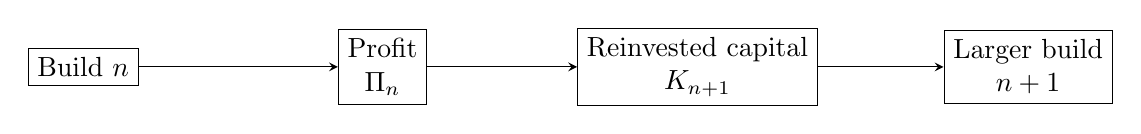
\begin{tikzpicture}[>=stealth]
\node[draw, rectangle, align=center] (b0) at (0,0) {Build $n$};
\node[draw, rectangle, align=center] (p) at (3.8,0) {Profit\\$\Pi_n$};
\node[draw, rectangle, align=center] (r) at (7.8,0) {Reinvested capital\\$K_{n+1}$};
\node[draw, rectangle, align=center] (b1) at (12.0,0) {Larger build\\$n+1$};
\draw[->] (b0) -- (p);
\draw[->] (p) -- (r);
\draw[->] (r) -- (b1);
\end{tikzpicture}
\end{figure}

\begin{remark}
The interview does not justify a technical treatment of 1031 law. All we need here is the strategic claim made by the speaker herself: rolling gains forward reduces current tax drag and leaves more capital available for the next project.
\end{remark}

Only after this scaling beat does the lecture return to its closing advice for the younger generation. Hard work, focus, and knowing the goal are not free-floating virtues in this section. They sit at the end of a concrete economic loop.

\section{Rejection, Reset, and Entrepreneurial Longevity}

The lecture then performs a necessary reset. The host briefly recaps what has just happened: the first homeowner was a former model turned real-estate developer in Los Angeles, a multimillionaire, and even the presence of her son is read as part of the lesson, since financial habits are already being transmitted across generations. That summary could have let the episode glide forward too easily. Instead, the transcript takes us back outside and shows refusals.

This matters. The lecture wants us to feel that access to wealthy people is scarce, contingent, and sometimes flatly denied. Several doors close. Privacy is asserted. Time runs out. The host's frustration surfaces. By the time the next accepted interview arrives, the narrative has been made costly again.

That next case takes place beside a Porsche and shifts immediately into business survival. The speaker says he started in software engineering, then turned toward marketing, and has now run his agency for nine years:
\begin{equation}
\tau_{\text{agency}} = 9\ \text{years}.
\end{equation}
The host's framing question is sharp: if most businesses fail, what actually prevents entrepreneurial longevity from collapsing under mistakes, slow sales, and the psychological damage of disappointment?

The answer is built from failure rather than glamour. The speaker says he ran a startup, failed to make it the multi-billion-dollar company he expected, and even though it was eventually acquired, that acquisition was not treated as the original dream fulfilled. This is a subtle but important beat. The lecture is not teaching that every outcome is secretly a victory. It is teaching that one disappointing outcome need not end the trajectory.

We can summarize the logic as a persistence-and-decision sequence:
\begin{enumerate}
\item A failure or weak period occurs.
\item One does not convert that local event into a total judgment on oneself.
\item One keeps moving forward.
\item One makes the next decision quickly.
\item One returns to execution before overthinking can harden into paralysis.
\end{enumerate}
The speaker's emphasis on decision speed is not decorative. It is one of the lecture's recurring structural ideas: time compounds, but so does delay. Capital compounds in the first case; here hesitation compounds.

The closing question about owning a Porsche one day might look lighter, but it preserves an important rhythmic feature of the lecture. Dream objects are never left as pure symbols of vanity. They are tied back to work, investment, saving, and childhood desire disciplined over time. The host then recaps again: software engineer, then marketer, then business mogul. We have moved from risk and reinvestment to survival and decision speed, and the chapter is now ready to escalate.

\section{Calabasas: Influence, Faith, and the Architecture of Scale}

The Calabasas segment begins with the same visual threshold as before: another expensive house, another driveway, another owner who has to be approached and persuaded. But once access is granted, the lecture turns quickly away from display and toward family history. The speaker says, in the transcript's rendering, that he was born in ``Columbia,'' came to the United States at six, and then saw his parents' dream collapse into a nightmare when the family home was raided and both parents went to jail.

This biographical turn is not incidental. The lecture is preparing the reader for a particular theory of scale, one rooted not merely in opportunity but in pressure and responsibility. At ten, the speaker says he promised his father he would take care of the house. At fifteen, he became in effect the head of household and started working early. Only after that pressure has been established does the lecture ask for the business structure that followed.

Now the case becomes quantitative:
\begin{align}
\tau_{\text{home security}} &= 25\ \text{years}, &
\tau_{\text{solar}} &= 1.5\ \text{years},\\
\operatorname{rank}_{\text{Inc5000}}(\text{solar company}) &= 20, &
R_{\text{this year}} &= \$2.0\times 10^8.
\end{align}
Again, these are speaker claims and should remain attributed as such. But they perform an important narrative function. Once the annual business volume reaches the order of two hundred million dollars, the host is entitled to ask not merely how the speaker survived, but how he scaled.

The first answer is influence. To bring in good people, they have to believe in you. The dream must be large enough that other people's dreams can fit inside it. This is already a theory of organization. Yet the lecture does not stop there. It asks what operational move makes such influence credible in the first place.

\subsection{Question \& Answer}

\paragraph{Question.} What does ``faith'' mean in business terms?

\paragraph{Answer.} The lecture gives a remarkably concrete definition: faith is taking action before you have what you need. The example is practical and memorable. The speaker bought the minivan before he had the people to fill it. In a cautious formalization we may write
\begin{equation}
a_t > 0 \qquad \text{while} \qquad r_t < r^\ast,
\end{equation}
where \(a_t\) is committed action, \(r_t\) is presently available resource, and \(r^\ast\) is the imagined threshold of readiness.

The lecture's point is that the ordinary order is reversed. One does not first wait until resources are complete and then act. One acts, and the action itself changes the state of the system. The sequence is:
\begin{enumerate}
\item Act before the resource picture feels complete.
\item Convert intention into commitment.
\item Let commitment raise what the speaker calls the necessity level.
\item Let necessity increase urgency.
\item Let urgency force recruitment, execution, and follow-through.
\end{enumerate}
This is the setting in which the speaker also says that low stress is low performance. The line should remain a maxim rather than a theorem, but its strategic content is plain: he deliberately places himself in pressure situations because he believes pressure untaps ability that comfort leaves dormant.

The passage then turns, with almost no wasted motion, from commitment to sales. The speaker says that when he sold home security door to door, he filled himself with conviction by reading about home invasions and fire accidents. The effect was not simply informational. It was psychological. It raised his confidence in the value of what he was selling, and that conviction altered his capacity to persuade. A compact rendering is
\begin{equation}
c_A > c_B \;\Rightarrow\; \mathcal{I}(A\to B)\text{ favors }A,
\end{equation}
where \(c\) denotes certainty and \(\mathcal{I}(A\to B)\) denotes the direction of influence from seller to buyer. The lecture immediately explains the meaning: people do not first need to believe the proposition; they need to believe that the speaker believes it. Everything is a transfer of belief.

At this point the lecture's architecture of scale is complete. It begins in family pressure, becomes commitment before readiness, becomes urgency, becomes recruitment and execution, and then becomes sales through conviction.

\section{Money Discipline, Motivated Ambition, and the Family Tree}

The final movement of the lecture narrows the lens. After two hundred million dollars in annual business volume, after influence, faith, urgency, and sales, the speaker is asked for the best financial advice he has ever received. The answer is almost austere in its simplicity: split the check three ways.

If \(C\) is one incoming check, then the rule may be written
\begin{align}
C &= C_{\text{live}} + C_{\text{tax/sav}} + C_{\text{reserve}},\\
C_{\text{live}} &\approx C_{\text{tax/sav}} \approx C_{\text{reserve}} \approx \frac{C}{3}.
\end{align}
The middle bucket should remain combined, just as the transcript gives it: IRS and savings together. The reserve account is the decisive term. It is to be treated as if it does not exist. That is the behavioral device that makes the formal split economically real.

A second schematic is useful here because the lecture wants this final rule to be repeatable, almost mechanical.

\begin{figure}
\centering
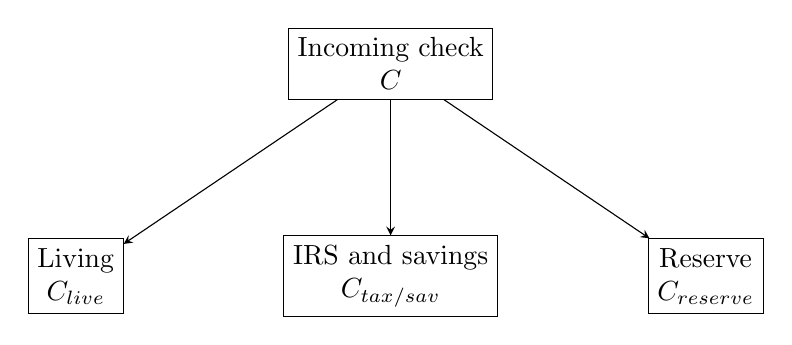
\begin{tikzpicture}[>=stealth]
\node[draw, rectangle, align=center] (c) at (0,0) {Incoming check\\$C$};
\node[draw, rectangle, align=center] (l) at (-4,-2.7) {Living\\$C_{\text{live}}$};
\node[draw, rectangle, align=center] (t) at (0,-2.7) {IRS and savings\\$C_{\text{tax/sav}}$};
\node[draw, rectangle, align=center] (r) at (4,-2.7) {Reserve\\$C_{\text{reserve}}$};
\draw[->] (c) -- (l);
\draw[->] (c) -- (t);
\draw[->] (c) -- (r);
\end{tikzpicture}
\end{figure}

The lecture explains why this matters. Life and pain are inseparable, and the reserve account exists to carry the household through those inevitable periods. That observation allows us to connect the end of the chapter back to its middle. Earlier, pressure was deliberately created to draw out action. Here, discipline is deliberately created to absorb future shocks. One doctrine produces motion; the other produces resilience.

The section then makes a turn that is easy to flatten if we are not careful. The speaker says he liked nice things. He wanted to stand out, wanted to be rare, and wanted, at twenty-one, to be the first in his city driving a Mercedes convertible rather than waiting until twenty-eight, when everybody would have one. This is not offered as an excuse for reckless consumption. It is offered as a description of motivated ambition. Luxury desire is acknowledged, but it is fenced inside the three-bucket rule.

The last line gathers the whole lecture into a single social claim: you do not come from a rich family, but a rich family can come from you. That is the proper end point. The cars and houses were never the real conclusion. The real conclusion is that repeated decisions about risk, reinvestment, effort, persuasion, and reserves can change the direction of a family line.

\section{Summary}

The lecture opens with spectacle, but it uses spectacle only to draw us into method. Wealth is made into a field site. From there the first homeowner gives us risk, self-belief, a concrete project profit, and the reinvestment loop by which one profitable build can finance a larger one, especially when tax drag is deferred. The next movement interrupts success with refusal and then rebuilds momentum through a case about entrepreneurial longevity, where failure is answered by continued motion and fast decisions rather than self-condemnation.

The Calabasas interview then pushes the argument further. We are given biography under pressure, a nine-figure scale claim, a theory of influence, a precise operational definition of faith as action before readiness, and a sales doctrine centered on certainty as a transferable force. The chapter finally narrows from company scale to household order: split the check, protect the reserve, let ambition remain motivating but bounded, and treat wealth as something that can redirect a lineage rather than merely decorate a moment.

If we compress the lecture to its strongest mathematical spine, we obtain four linked rules. Profit compounds when it is rolled forward. Scale deepens when commitment precedes comfort. Persuasion strengthens when conviction is internally settled. Family transformation becomes plausible when disciplined allocation is repeated long enough. The host does not announce these laws at the start. He walks us to them, one door at a time.